\section{Experiments}
\label{experiments}
In this section, we conduct experiments to show the performance and scalability of \texttt{BeeSwarm}. We use a Department of Energy (DOE) code, Flecsale \cite{charest2017flexible}, as an example software development project. We deploy \texttt{BeeSwarm} on Travis CI test environment and use Chameleon Cloud \cite{mambretti2015next} as the computation back-end for the scalability tests. The Chameleon Cloud is an OpenStack-based cloud computing platform that offer bare-metal access to all computing nodes. It is currently deployed at University of Chicago and the Texas Advanced Computing Center with total 650 multi-core nodes. We conduct our test on the nodes located at University of Chicago. 

\subsection{Modified Travis CI script}
In this section, we show a sample modified Travis CI script for Flecsale that has \texttt{BeeSwarm} scalability test enabled (\textbf{Listing 1}). Line 1 - 12 are the original Flecsale test code on Travis CI. To enable \texttt{BeeSwarm} scalability test, we only need to add less than 10 lines of simple code (line 13 - 18). The original CI script include building a Docker image  (line 9), running the Docker image (line 10) to correctness test scrips, and push the image to DockerHub if the test was successful (line 12). We add the \texttt{BeeSwarm} configuration and launching scripts after the image is successfully pushed onto the DockerHub. We obtain and install \texttt{BeeSwarm} in line 13 and 14. We add necessary environment variables (for OpenStack and \texttt{BeeSwarm}) in line 15. The scalability test is launched using a simple command in line 16. We add a 120 minutes timeout here since Travis CI would kill a job if a command runs more than 10 minutes by default and a scalability test usually needs more time than that. The actual timeout length can be set based on need of a specific application. Finally, we run the output parser in line 17 followed by pushing scalability test result to original code repository in line 18. It can be seem that with minimum modification current CI scripts can easily enable scalability test through \texttt{BeeSwarm} and the scalability test code is highly portable across any kind of CI service platforms.

\lstset{numbers=left,
xleftmargin=1.5em,
frame=single,
framexleftmargin=2em}


\lstset{language=Java}
\begin{lstlisting}[escapechar=!,
				   caption= Example Travis CI script (\texttt{.travis.yml}) for Flecsale with \texttt{BeeSwarn} scalability test. Highlighted part shows that only simple modifications are required to enable autonomic scalability test.]
language: cpp
sudo: required
services:
 - docker
before_install:
 - git fetch --unshallow 
 - git fetch --tags
script:
 - docker build -t <img> <dockerfile> 
 - docker run <img> <correctness_test>
after_success:
 - docker push <img>
 - !\hl{git clone https://github.com/lanl/BEE.git \&\& cd ./BEE}!
 - !\hl{./install\_on\_travis.sh}!
 - !\hl{source openrc.sh}!
 - !\hl{travis\_wait 120 bee\_ci\_launcher.py -l flecsale}!
 - !\hl{output\_parser.py}!
 - !\hl{push\_results\_to\_repo.sh}!
\end{lstlisting}

\begin{comment}

\end{}
\begin{lstlisting}[language=yaml]
language: cpp
sudo: required
services:
- docker
env:
  matrix:
    - DISTRO=ubuntu_mpi BUILD_TYPE=Debug DOCKERHUB=true
before_install:
 - git fetch --unshallow && git fetch --tags
script:
  - if [[ ${CC} != gcc ]]; then TAG="_${CC}"; fi
  - if [[ ${TRAVIS_BRANCH} != stable ]]; then TAG="${TAG}_master"; fi
  - cp -vr docker ${HOME}/docker
  - sed -i "1s/fedora_serial/${DISTRO}${TAG}/" ${HOME}/docker/Dockerfile
  - cd ../../
  - cp -r ${TRAVIS_REPO_SLUG} $HOME/docker
  - docker build --build-arg BUILD_TYPE=${BUILD_TYPE} 
     --build-arg CC=${CC} 
     --build-arg CXX=${CXX}
     --build-arg CI=${CI}
     --build-arg TRAVIS=${TRAVIS} 
     --build-arg TRAVIS_OS_NAME=${DISTRO}
     --build-arg TRAVIS_BRANCH=${TRAVIS_BRANCH} 
     --build-arg TRAVIS_JOB_NUMBER=${TRAVIS_JOB_NUMBER}
     --build-arg TRAVIS_PULL_REQUEST=${TRAVIS_PULL_REQUEST} 
     --build-arg TRAVIS_JOB_ID=${TRAVIS_JOB_ID}
     --build-arg TRAVIS_TAG=${TRAVIS_TAG} 
     --build-arg TRAVIS_REPO_SLUG=${TRAVIS_REPO_SLUG}
     --build-arg TRAVIS_COMMIT=${TRAVIS_COMMIT}
     -t ${TRAVIS_REPO_SLUG}:${DISTRO}${TAG} ${HOME}/docker/ 
   - docker run -d ${TRAVIS_REPO_SLUG}:${DISTRO}${TAG} /bin/bash
after_success:
   - if [[ ${DOCKERHUB} = true && ${DOCKER_USERNAME} && ${DOCKER_PASSWORD} && ${TRAVIS_PULL_REQUEST} == false && ${TRAVIS_BRANCH} == master && ${CC} = gcc ]]; then
      docker login -u="$DOCKER_USERNAME" -p="$DOCKER_PASSWORD";
      docker push "${TRAVIS_REPO_SLUG}:${DISTRO}${TAG}";
      cd ${HOME}
      git clone https://${GH_TOKEN}@github.com/lanl/BEE_Private.git && cd ./BEE_Private
      ./install_on_travis.sh
      source ${HOME}/build/${TRAVIS_REPO_SLUG}/bee_scalability_test/CH-819321-openrc.sh
      export PATH=$(pwd)/bee-launcher:$PATH
      export PATH=$(pwd)/travis_ci:$PATH
      export PATH=${HOME}/build/${TRAVIS_REPO_SLUG}/bee_scalability_test:$PATH
      cd ${HOME}/build/${TRAVIS_REPO_SLUG}/bee_scalability_test
      travis_wait 120 bee_ci_launcher.py -l flecsale -r $OS_RESERVATION_ID
      output_parser.py
      push_results_to_repo.sh
    fi
compiler:
  - gcc
\end{lstlisting}
\end{comment}

\subsection{Performance of \texttt{BeeSwarm}}
\begin{comment}


\begin{figure}[h]
    \centering
    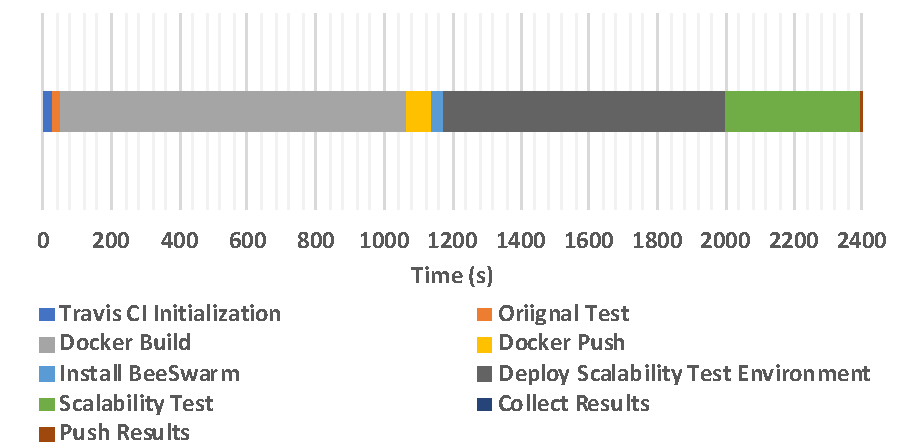
\includegraphics[width=0.5\textwidth]{figures/perf.pdf}
    \caption{Time breakdown of CI for Flecsale with \texttt{BeeSwarm} Scalability Test}
    \label{perf}
\end{figure}
\end{comment}
In order to evaluate the performance of \texttt{BeeSwarm}, we discuss the overhead of launching \texttt{BeeSwarm} and the scalability of \texttt{BeeSwarm} for large-scaled test.

\subsubsection{Overhead of \texttt{BeeSwarm}}
\textbf{Fig. \ref{breakdown}} shows the time breakdown of CI for Flecsale with \texttt{BeeSwarm} scalability test including the original correctness test on Travis CI and one set of multi-node scalability tests using texttt{BeeSwarm}. The scalability test involves different execution configurations that range from 1 process to 128 processes. We can see the major overhead of \texttt{BeeSwarm} comes from deploying the scalability test environment. This is mainly caused by long instance launching time on Chameleon cloud. However, since CI tests are usually not on the critical path of applications' development process, the extra time cost brings negligible impact to developers.   %\paul{Are their any expectation on specifying software version of hardware details?}


\begin{comment}
\begin{table}[h]
\centering
\caption{An Example Time Breakdown of CI with Scalability Test. \textcolor{red}{JIEYANG, this part is quite misleading, You have  1223.88s+42.89s(overhead?)  in this table, but in the figure 4, you are putting 820s. Reviewers will challenge this. Please change. I understand that may come from different applications, but they should be either specified (point out the difference in configuration of platform or application setup)  or kept everything just consistent.}}
\label{time-breakdown}
\begin{tabular}{c|c|c|c}
           & \begin{tabular}[c]{@{}c@{}}Correctness \\ Test\end{tabular} & \begin{tabular}[c]{@{}c@{}}Scalability \\ Test\end{tabular} & \begin{tabular}[c]{@{}c@{}}\texttt{BeeSwarm} \\ Overhead\end{tabular} \\ \hline
Time (s)   & 1013.12                                                     & 1223.88                                                     & 42.89                                                        \\ \hline
Percentage & 44.4\%                                                      & 53.7\%                                                      & 1.9\%                                                       
\end{tabular}
\end{table}
\end{comment}
\begin{figure}[h]
    \centering
    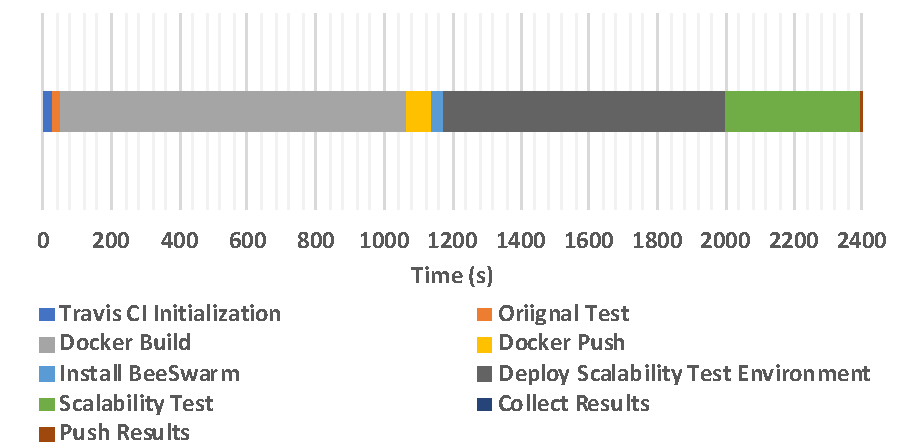
\includegraphics[width=0.5\textwidth]{figures/perf.pdf}
    \caption{Time breakdown of an example CI test with \texttt{BeeSwarm} scalability test.}
    \label{breakdown}
\end{figure}

\subsubsection{Scalability of \texttt{BeeSwarm} } % I think we don't need to separately 
\begin{figure}[h]
    \centering
    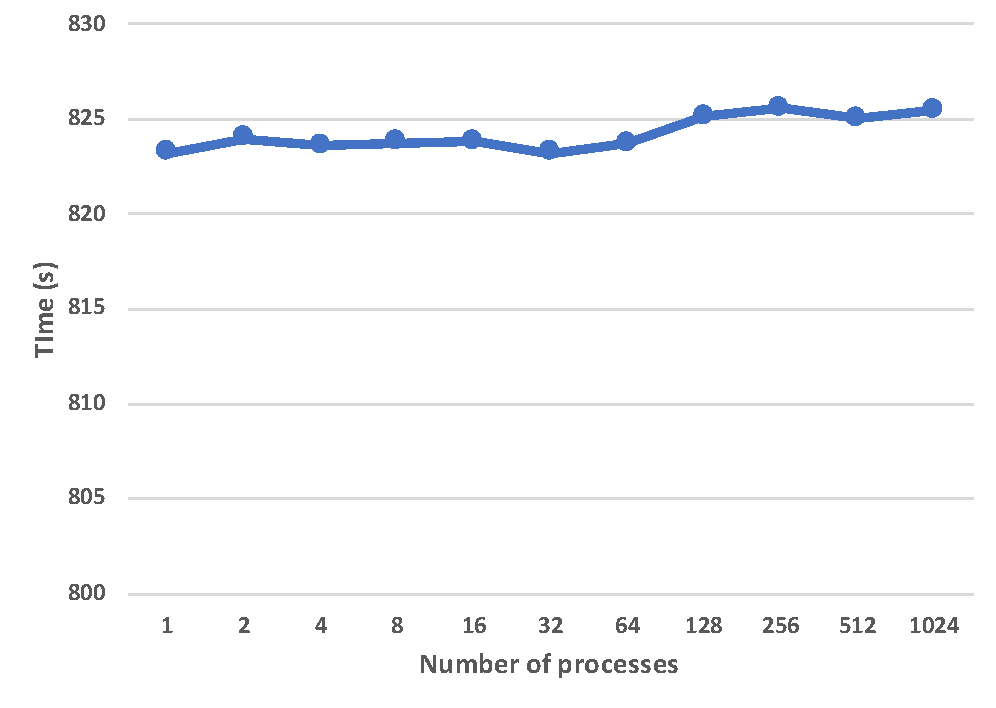
\includegraphics[width=0.45\textwidth]{figures/scalability.pdf}
    \caption{Scalability of deploying scalability test environment for \texttt{BeeSwarm}.}
    \label{scalability}
\end{figure}

Since BeeSwarm is designed for launching large-scaled parallel applications, the scalability of \texttt{BeeSwarm} itself is also very important. 
As we mentioned before, the main overhead of \texttt{BeeSwarm} comes from deploying the scalability test environment. \textbf{Fig. \ref{scalability}} shows the performance of deploying the scalability test environment for \texttt{BeeSwarm}. We test it with an increasing number of processes ranging from 1 to 1024. 
We run the scalability test on 16 instances on Chameleon cloud. Each instance has 64 cores. From \textbf{Fig. \ref{scalability}}, we can see the time cost is nearly constant (less than 900 seconds) as we increase the number of process. This indicate the scalability of \texttt{BeeSwarm} itself is very good.

%When the number of processes are greater than 64, \texttt{BeeSwarm} launches multiple instances. The time cost increases to about 1200 seconds and slightly increases with the number of instances. The sharp increase of time between launching one instance and two instances is because of the launching procedure of \texttt{BeeSwarm}. The scalability test environment that \texttt{BeeSwarm} deploys contains one master instance and zero or more worker instances. The master holds a working directory that is shared between workers, so the master instance must be launched first before workers. So, when we only need one instance only the master instance is launched. Otherwise, more worker instances need to be launched, taking extra time due to the dependency on the master instance. Beyond two instances, the time cost increases only slightly (4.9\% - 9.6\%, avg. 7.6\%). %\pat{you should probably quatify this here, what is slightly?}
%Worker instances do not have dependencies between each other, so they can be launched in parallel. The increase of time only comes from the extra configuration after each worker has launched.
%\texttt{BeeSwarm} shows good scalability performance on large scale scalability tests. %\pat{again should this be quantified?}

\subsection{Scalability Test Showcase}

\begin{figure}[h]
    \centering
    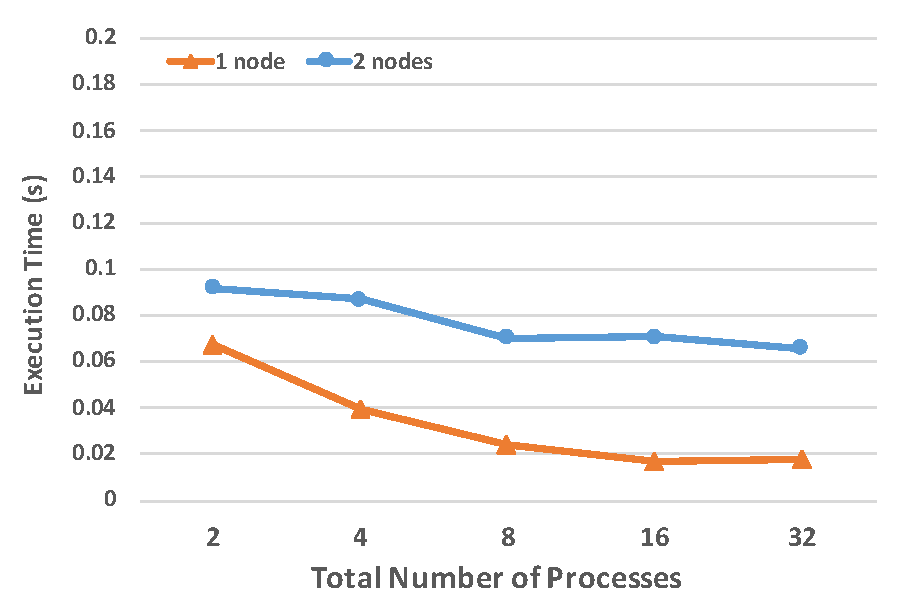
\includegraphics[width=0.45\textwidth]{figures/flecsale-result.pdf}
    \caption{The scalability test result of Flecsale.}
    \label{flecsale-result}
\end{figure}

We use Flecsale to showcase a sample scalability test using \texttt{BeeSwarm}. We configure it to run using 2 to 32 processes on one or two nodes. When using two nodes, we evenly divide the total number of processes among them (each has 1 to 16 processes). The file generated by \texttt{BeeSwarm} is in the comma separated values (CSV) file format, and we plotted the result data in \textbf{Fig. \ref{flecsale-result}}. %\trandles{Same comment here again about using colors on graphs}
Even with this simple test using \texttt{BeeSwarm}, we can observe some interesting behavior of Flecsale. We can see Flecsale gains better speedup (1.73x - 4.01x) on a single node environment compared to the speedup on two nodes (1.05x - 1.40x) given the same total number of processes. This may suggest that inter-node communication could be a performance bottleneck for Flecsale running on systems similar to Chameleon.


%However, the two node environment is more suitable for 64 processes compared to the single node.

This result can effectively give developers the scalability data of the application they are developing, so that they can make adjustment to their application in a more timely manner. Not only can the developer observe behavior of different processing schemes, but using \texttt{BeeSwarm} can help aid them to see performance improvement or degradation of their application as they push changes to the application. %\pat{I added the sentence before this comment} %\trandles{I worry that the claims about Flecsale scalability may be false given there's no discussion of interconnect, especially since you're using virtual machines.  Is this MPI or Legion using ethernet?  I don't think scalability will look like this on bare metal HPC nodes using IB or OPA with RDMA} %\pat{Can we make the point that this is an example and can't it be submitted to one of the other platforms?}